\documentclass[./chapters/design.tex]{subfiles}

\begin{document}
\section{Backend structure}
As mentioned previously, the project includes a backend component that
encompasses a significant portion of the content, which is why three team
members are dedicated to backend development. The objective of this section is
to provide an overview of the backend architecture and structure without delving
into extensive implementation details.
\\
Although I did not actively participate in the backend implementation, the team
collectively made decisions regarding its architecture and structure. Once the
application requirements were defined, the team realized that the backend could
be structured as either a monolithic application or a microservice architecture.
Ultimately, the team opted for a service-based structure due to the following
reasons:
\\
\begin{enumerate}[label = -]
	\item Simplified asynchronous development: With each service contained in a
	      separate repository, team members could focus on their respective projects
	      independently. This streamlined asynchronous work and reduced the
	      likelihood of conflicts arising.
	\item Faster CI/CD processes: Each repository has its own set of tests and
	      deployment processes. By separating each project, the time required to run
	      tests and deploy applications was significantly reduced, as less code
	      needed to be checked, compiled, and built.
\end{enumerate}
A service-based architecture typically involves communication between different
services or applications. This challenge is commonly addressed by implementing a
message queue, which allows backends to subscribe to and publish events.
\\[8pt]
Another important aspect about each backend service desing is that it has been
written using using an hexagonal architecture approach, combined with
domain-driven design.
\subsection{Api gateway}
The backend consists of multiple services, with each service having a specific
functionality. However, it is important that clients using this backend are
unaware of its internal structure. If clients were aware of each individual
domain and had to make requests accordingly, it would create an undesirable
dependency for the frontend.
\\[8pt]
To address this issue, the team implemented an API gateway as a solution. This
gateway acts as an intermediary, receiving requests from the frontend and
determining which service should handle each request. Additionally, the API
gateway handles user authentication for the frontend and ensures that only
authenticated requests are allowed, blocking unauthorized access.
\\[8pt]
The API gateway provides several advantages and is an optimal solution in terms
of scalability and migration management. Firstly, it simplifies the integration
process for all connected frontends by maintaining a consistent contract for
each request. Any changes made to the backend services will not directly impact
the frontends, as long as the contract remains intact. This allows for seamless
updates and modifications to the backend without disrupting the functionality of
the frontends.
\\[8pt]
Furthermore, the API gateway provides a layer of abstraction, shielding the
frontends from the complexities of the backend architecture. Even if there are
changes behind the API gateway, such as consolidating all microservices into a
monolithic structure, the frontends remain unaffected as long as the contract
between the API gateway and the frontends remains unchanged.
\\[8pt]
In summary, the implementation of the API gateway not only solves various
challenges but also offers a scalable and resilient solution that decouples the
frontends from the backend services, ensuring flexibility and ease of
maintenance in the long run.
\begin{figure}[H]
	\centering
	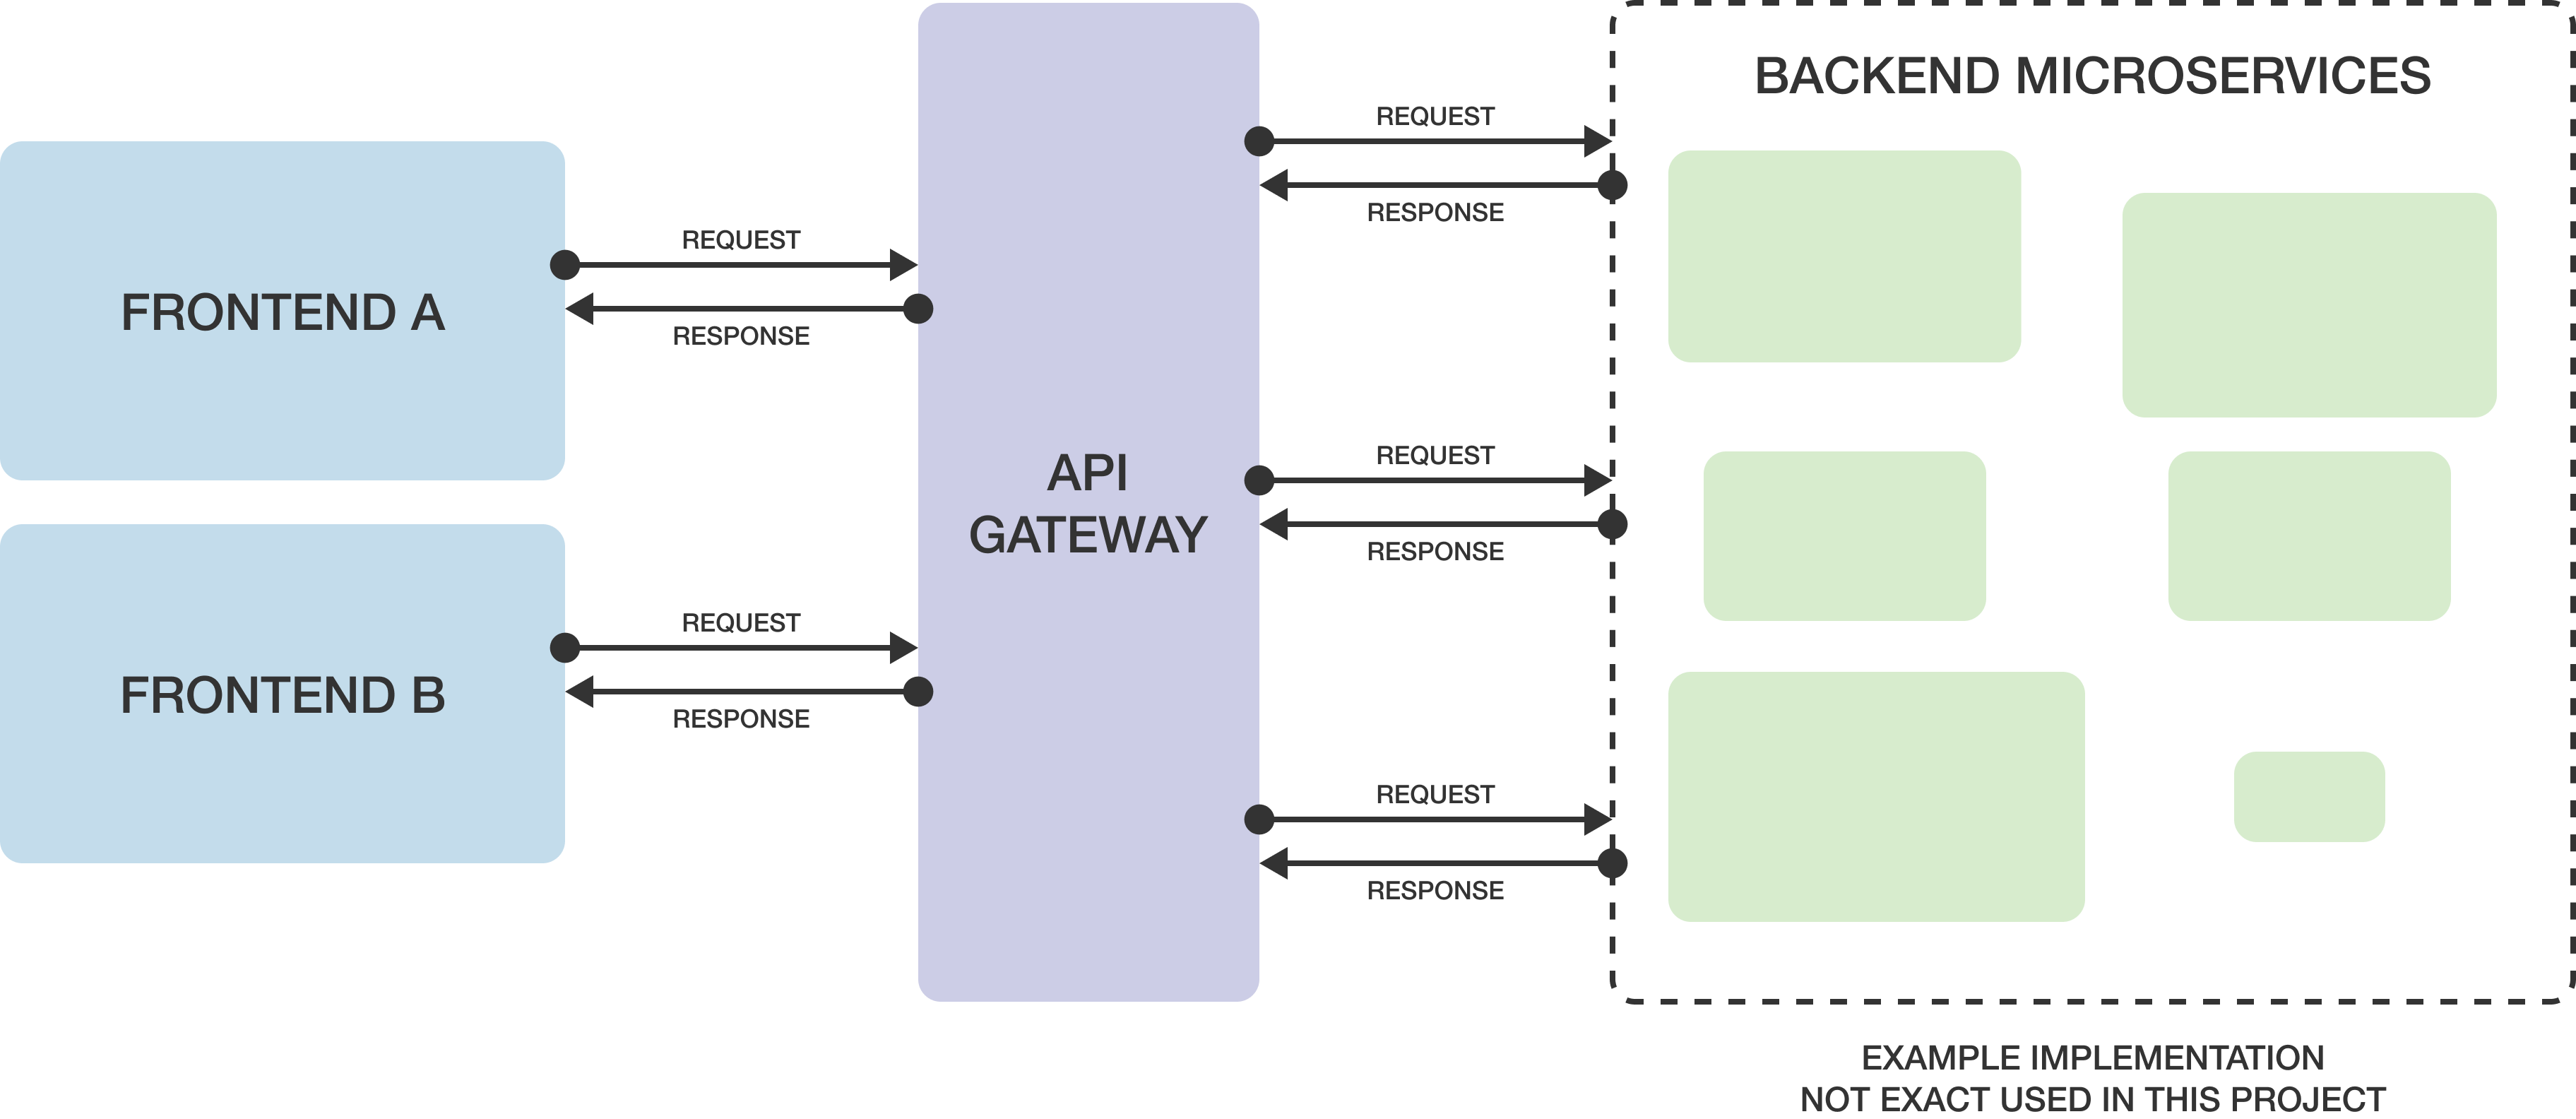
\includegraphics[width=\textwidth]{./assets/api-gateway.png}
	\caption{Example benefits of the API gateway}
\end{figure}
The above figure exemplifies the benefits of the API gateway. On the one hand,
we can have as many frontends as wanted connected to the gateway. It works as a
façade to what is behind. On the other hand, the microservices will also only
communicate with the gateway, satisfying the contract specified.
\subsection{Service-based architecture}
Opting for a service-based or microservice based architecture in the backend was
the idea that appeared more attractive to the team. As explained previously, it
provides a lot of benefits in terms of development, CI/CD, while allowing us to
apply other software architecture patterns such as hexagonal architecture.
\\
Even though all backends have been written in Java, which is the predominant
language known by the team members, each service could have been written in a
different language. Such features are helpful in an enviornment and team that
aspires for an scalable, easy to maintain, and robust ecosystem.
\\[8pt]
The microservices are as follows:
\begin{figure}[H]
	\centering
	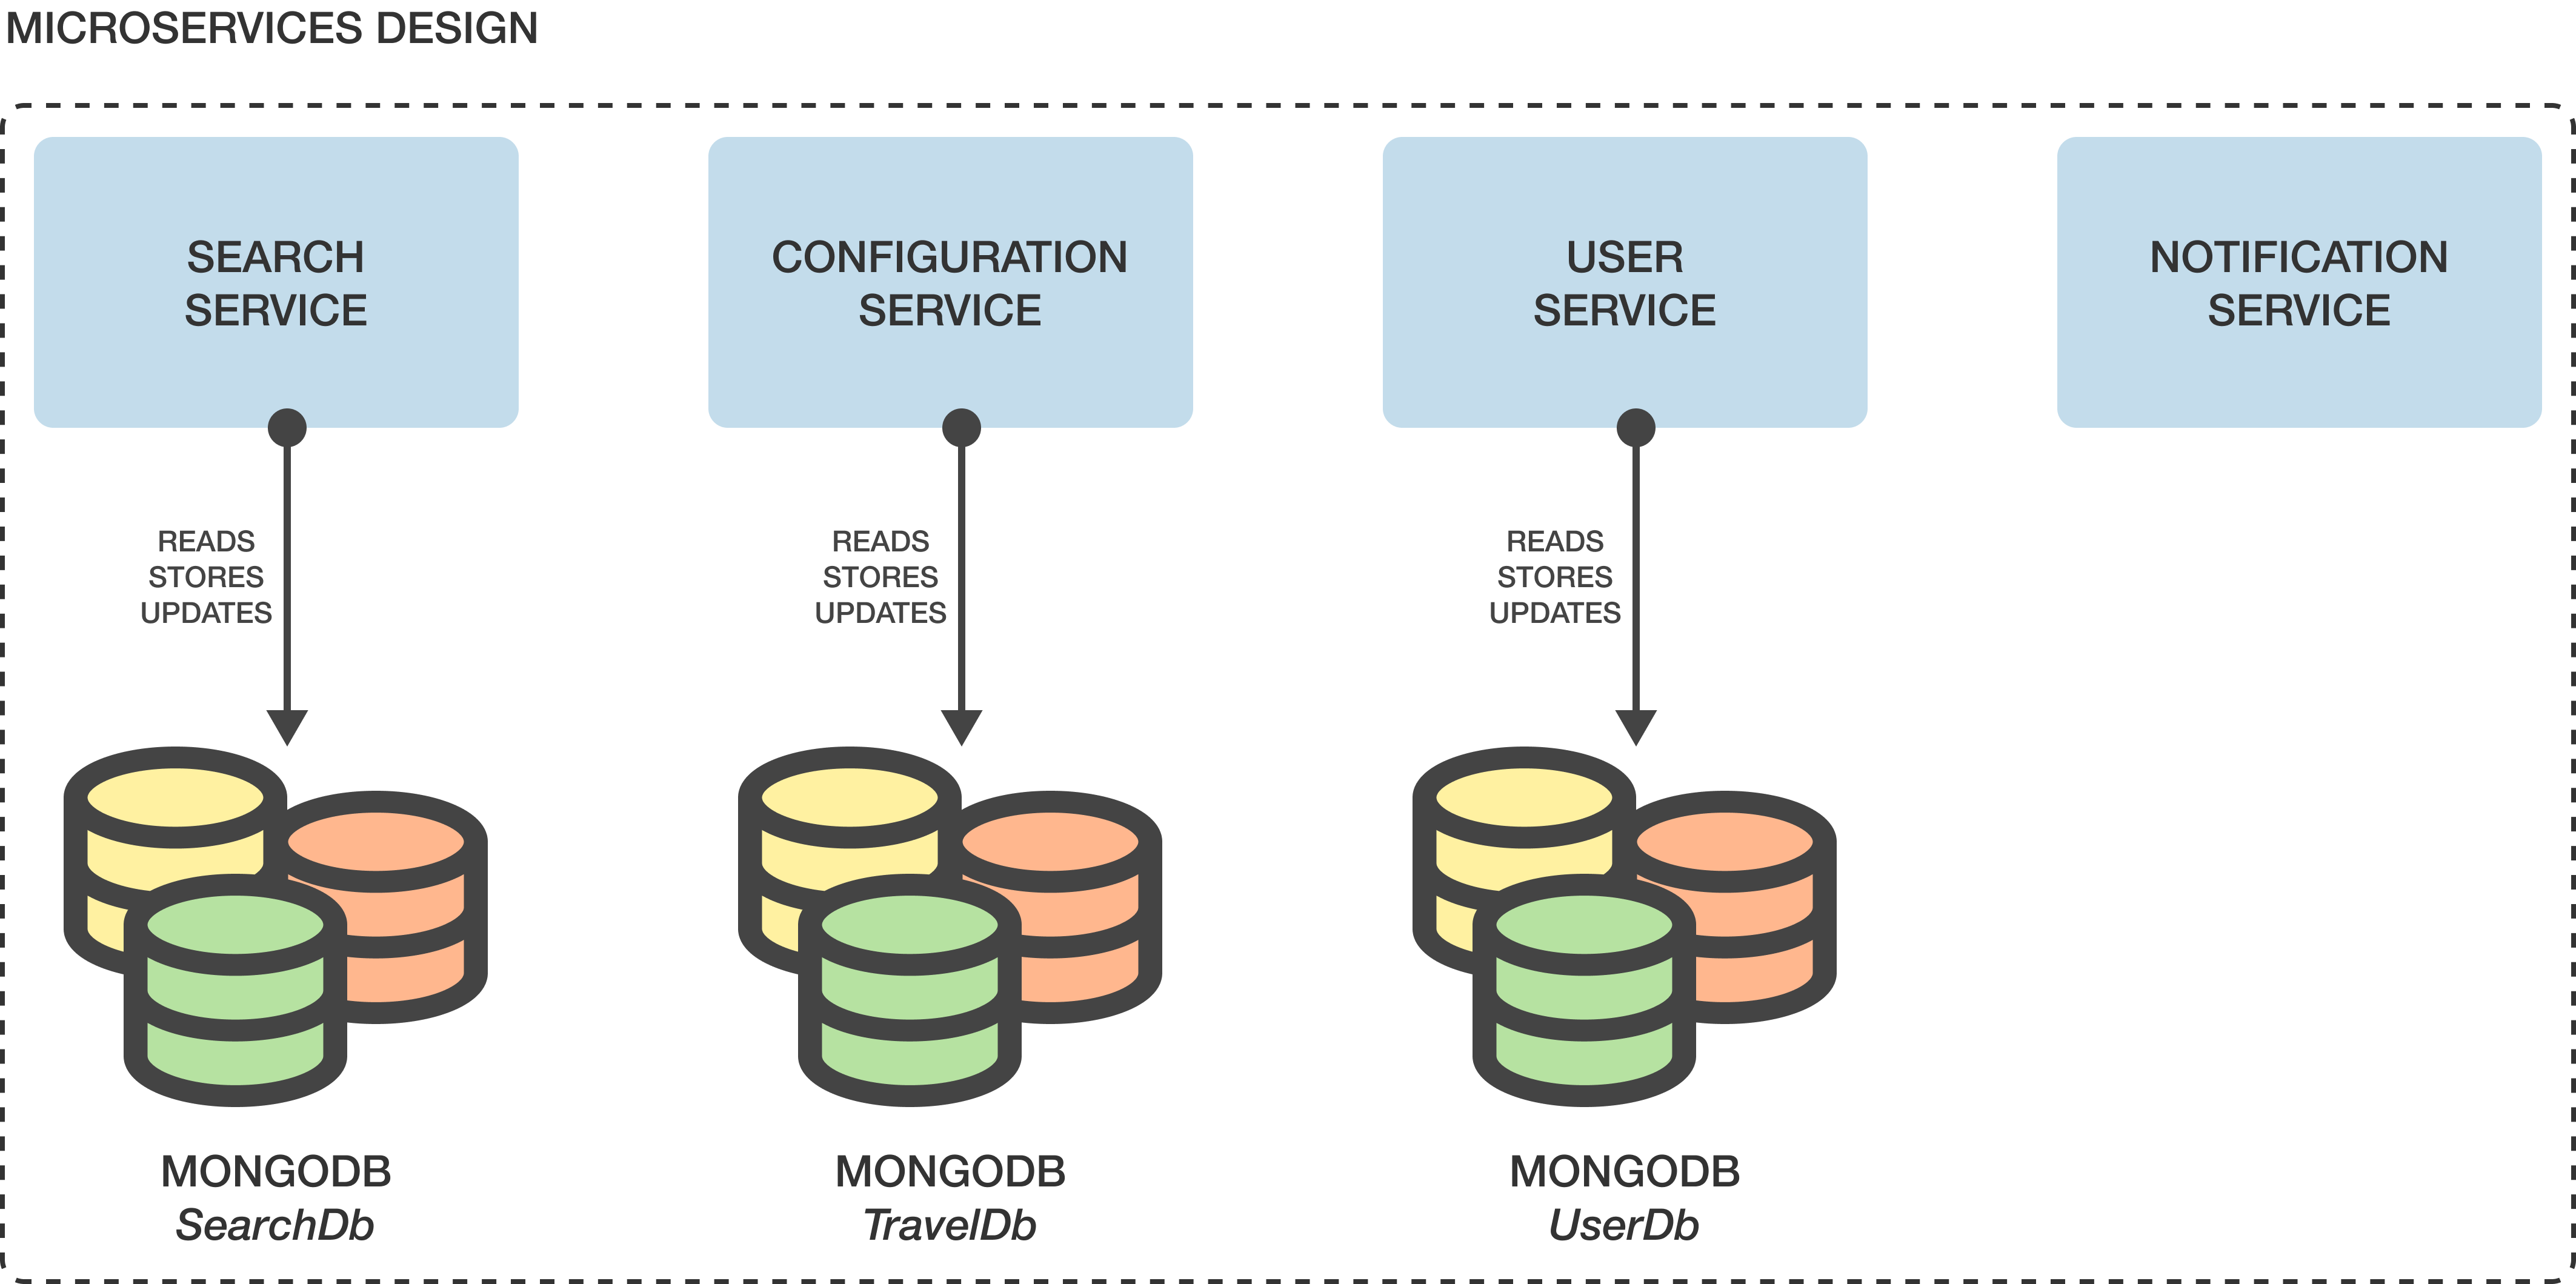
\includegraphics[width=\textwidth]{./assets/microservice-struct.png}
	\caption{Initial backend microservice structure}
\end{figure}
Without getting into much detail about the implementation of each backend, each
has its own database, all working within the same MongoDb cluster. It is common
to use a different database for each service when working with microservices.
\\
The function of each service is:
\begin{enumerate}[label = -]
	\item\textbf{Search service}. Responsible for executing the asynchronous job
	of searching for results of each travel alert.
	\item\textbf{Configuration service}. Responsible for managing the travels that
	a user can create.
	\item\textbf{User service}. Responsible for managing the user data. It
	provides the endpoints for registering, authentication and token refreshing.
	\item\textbf{Notification service}. Responsible for notifying the user through
	email or WhatsApp with the new travel alerts found.
\end{enumerate}
The goal of the API gateway is to hide this structure from the backend.
Therefore, if the gateway is added to the previous diagram, it is obtained:
\begin{figure}[H]
	\centering
	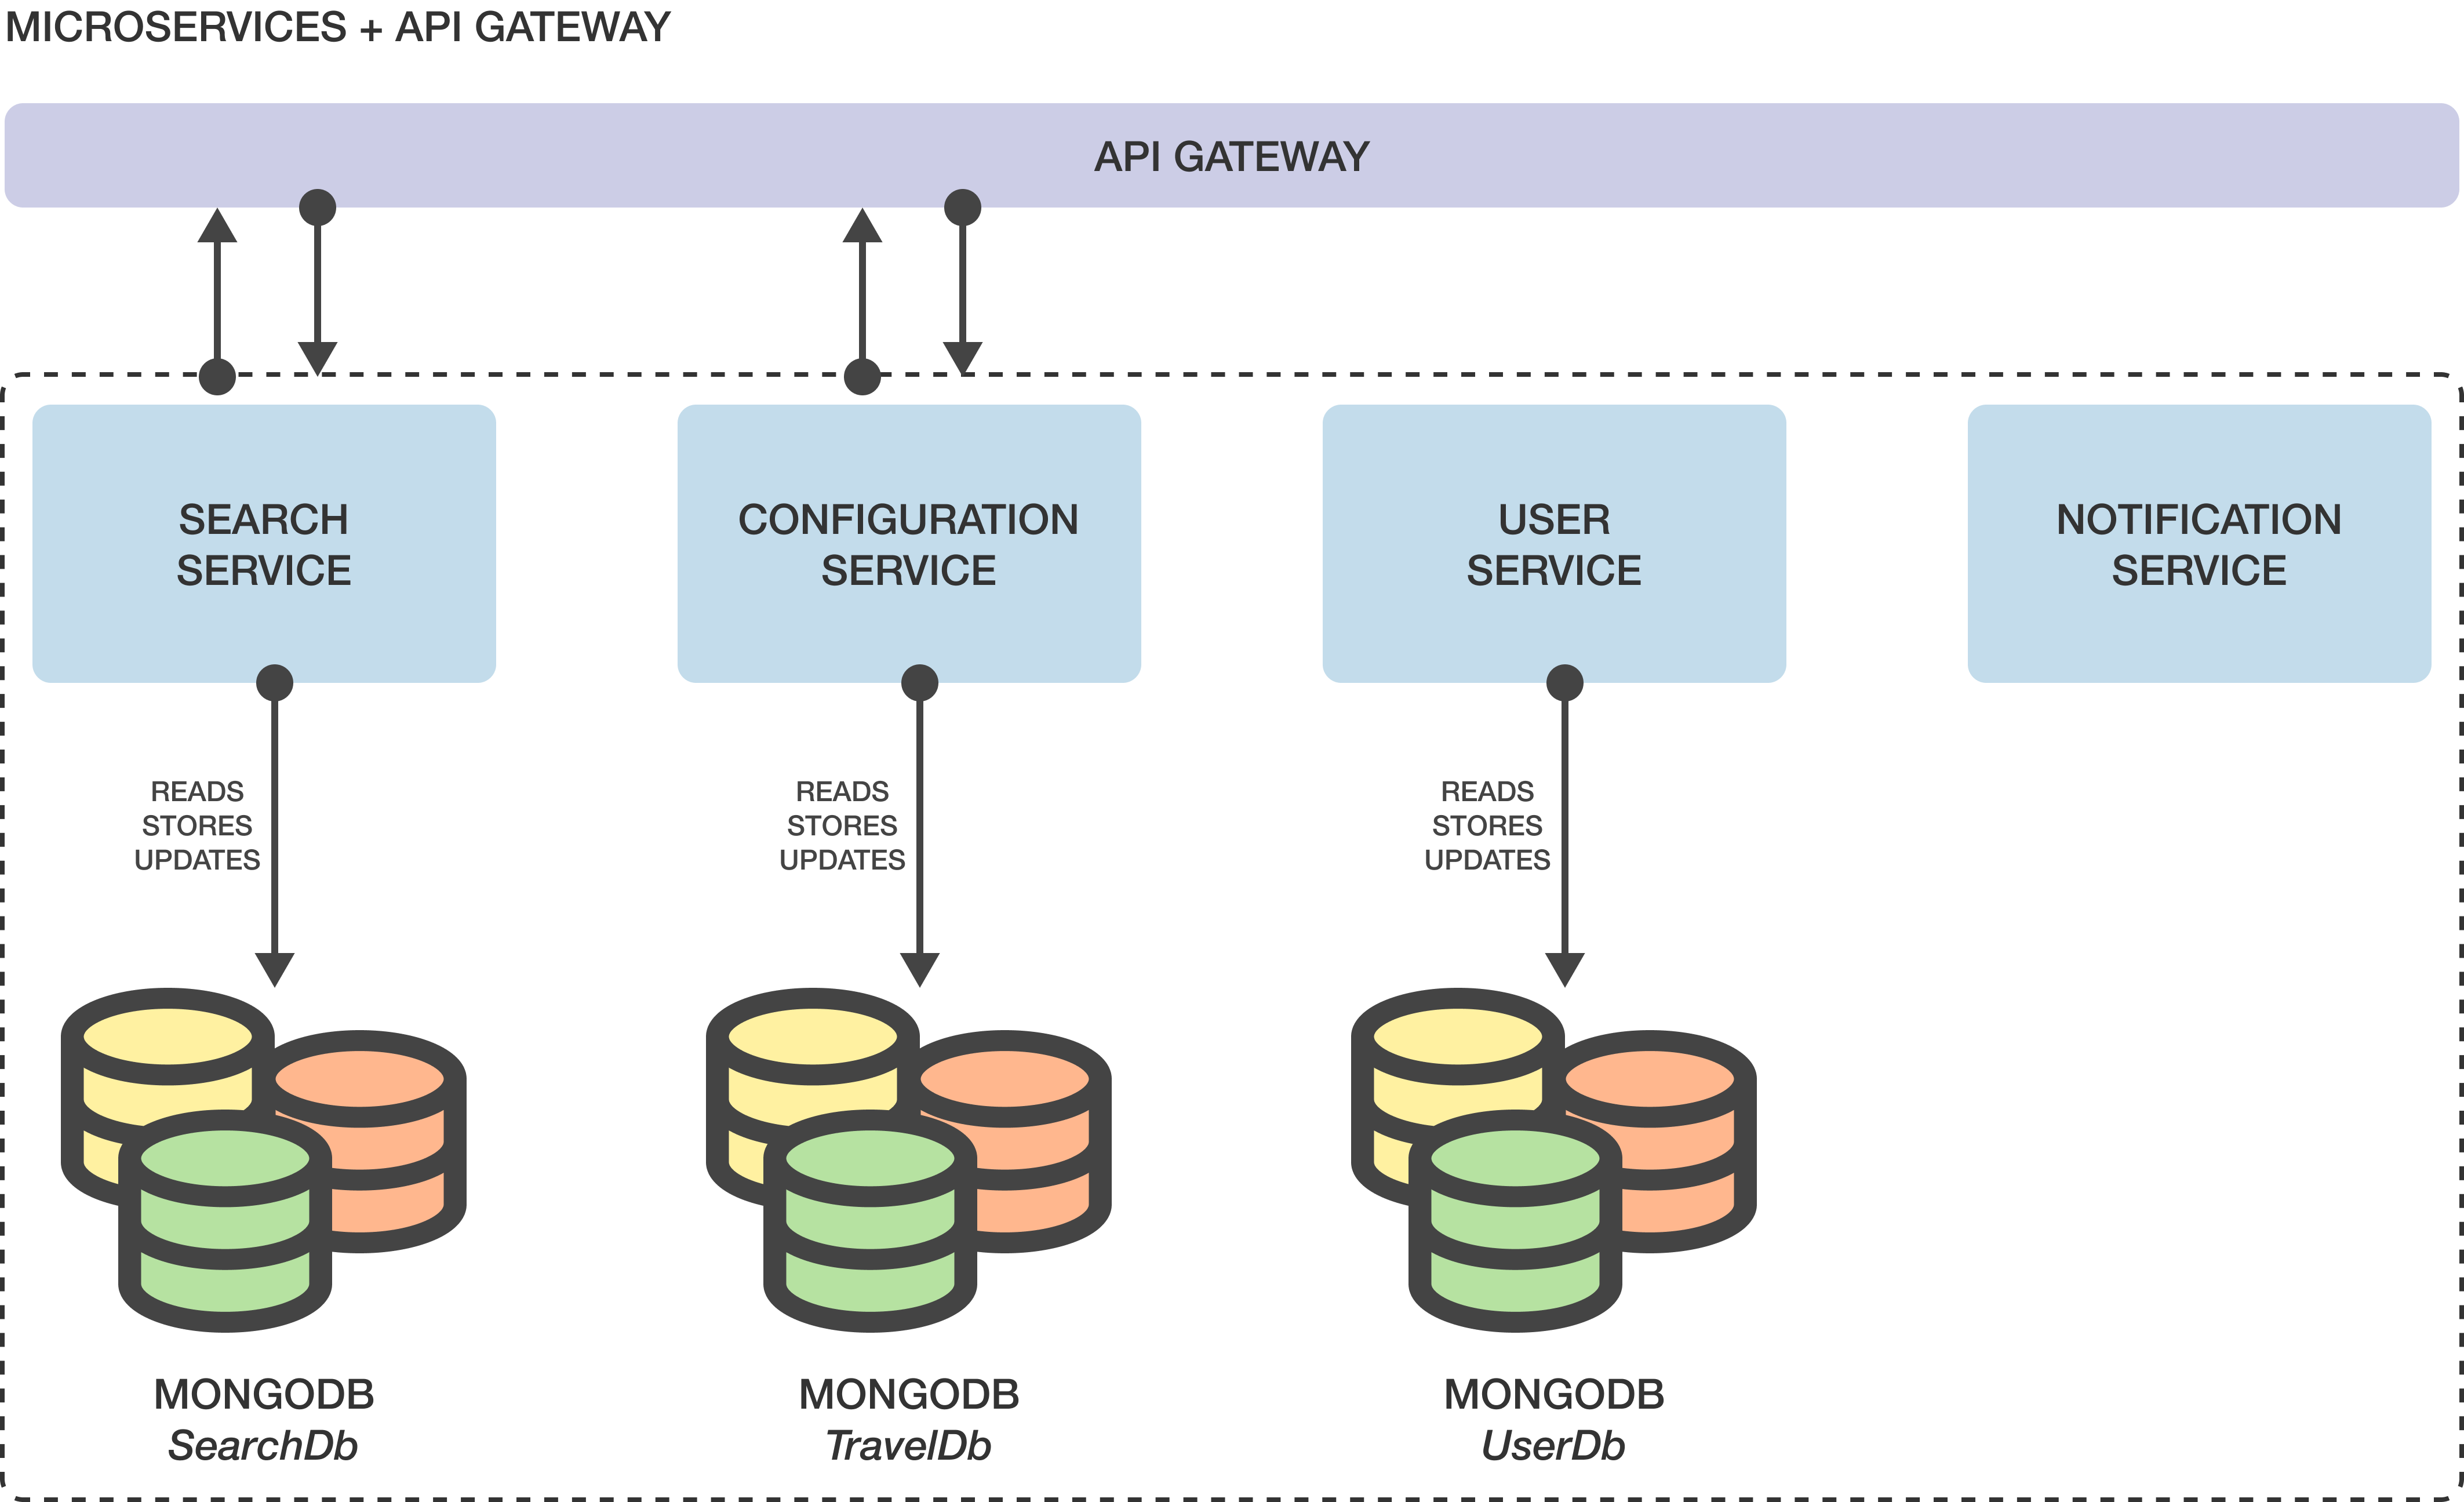
\includegraphics[width=\textwidth]{./assets/microservice-gateway-struct.png}
	\caption{Microservices connected with the gateway}
\end{figure}
As it can be seen in the figure above, the gateway only will send requests to
the user and configuration services. That is because the search service is made
to work internally and share the results to the other services.
\\
The gateway will forward authentication calls to the user service, i.e. requests
regarding registering and loggin in, or a webservice to refresh the
authentication token of a user. It will send the configuration of the travels to
the configuration service. This service will store all the travel alerts for the
user, as well as notifying the search service to start performing the required
search.
\subsection{Event driven architecture}
When the configuration service requests for a list of results to the searh
service, it could keep a connection between the two applications. However, this
behaviour is not performant at all, as the more requests there are, the more
blocked the applications will be. This is trabslated to an extremely poor
performance from our backend, as well as an extensive amount of resource usage.
\\
Therefore, the solution is to establish asynchronous communication between the
different backend applications. This approach enables a backend to send a
message to another backend without actively waiting for the response. Once the
response is received, the backend can take appropriate action. Meanwhile, the
sending backend can continue executing other tasks concurrently.
\\
By adopting an asynchronous communication model, backends can achieve better
efficiency and utilize their resources more effectively. Instead of blocking and
waiting for responses, backends can offload tasks to other components and
proceed with additional operations. This asynchronous nature enables backends to
maximize their throughput and responsiveness, leading to improved overall system
performance.
\\
Moreover, asynchronous communication allows for greater flexibility and fault
tolerance. If a backend receives a high volume of requests or experiences delays
in processing, the asynchronous approach ensures that other backends can
continue functioning independently, preventing bottlenecks and maintaining
system stability.
\\[8pt]
In order to achieve this asynchronous communication, the team has opted to use a
RabbitMq message broker for the backends. By adding the new broker, the schema
is updated as following:
\begin{figure}[H]
	\centering
	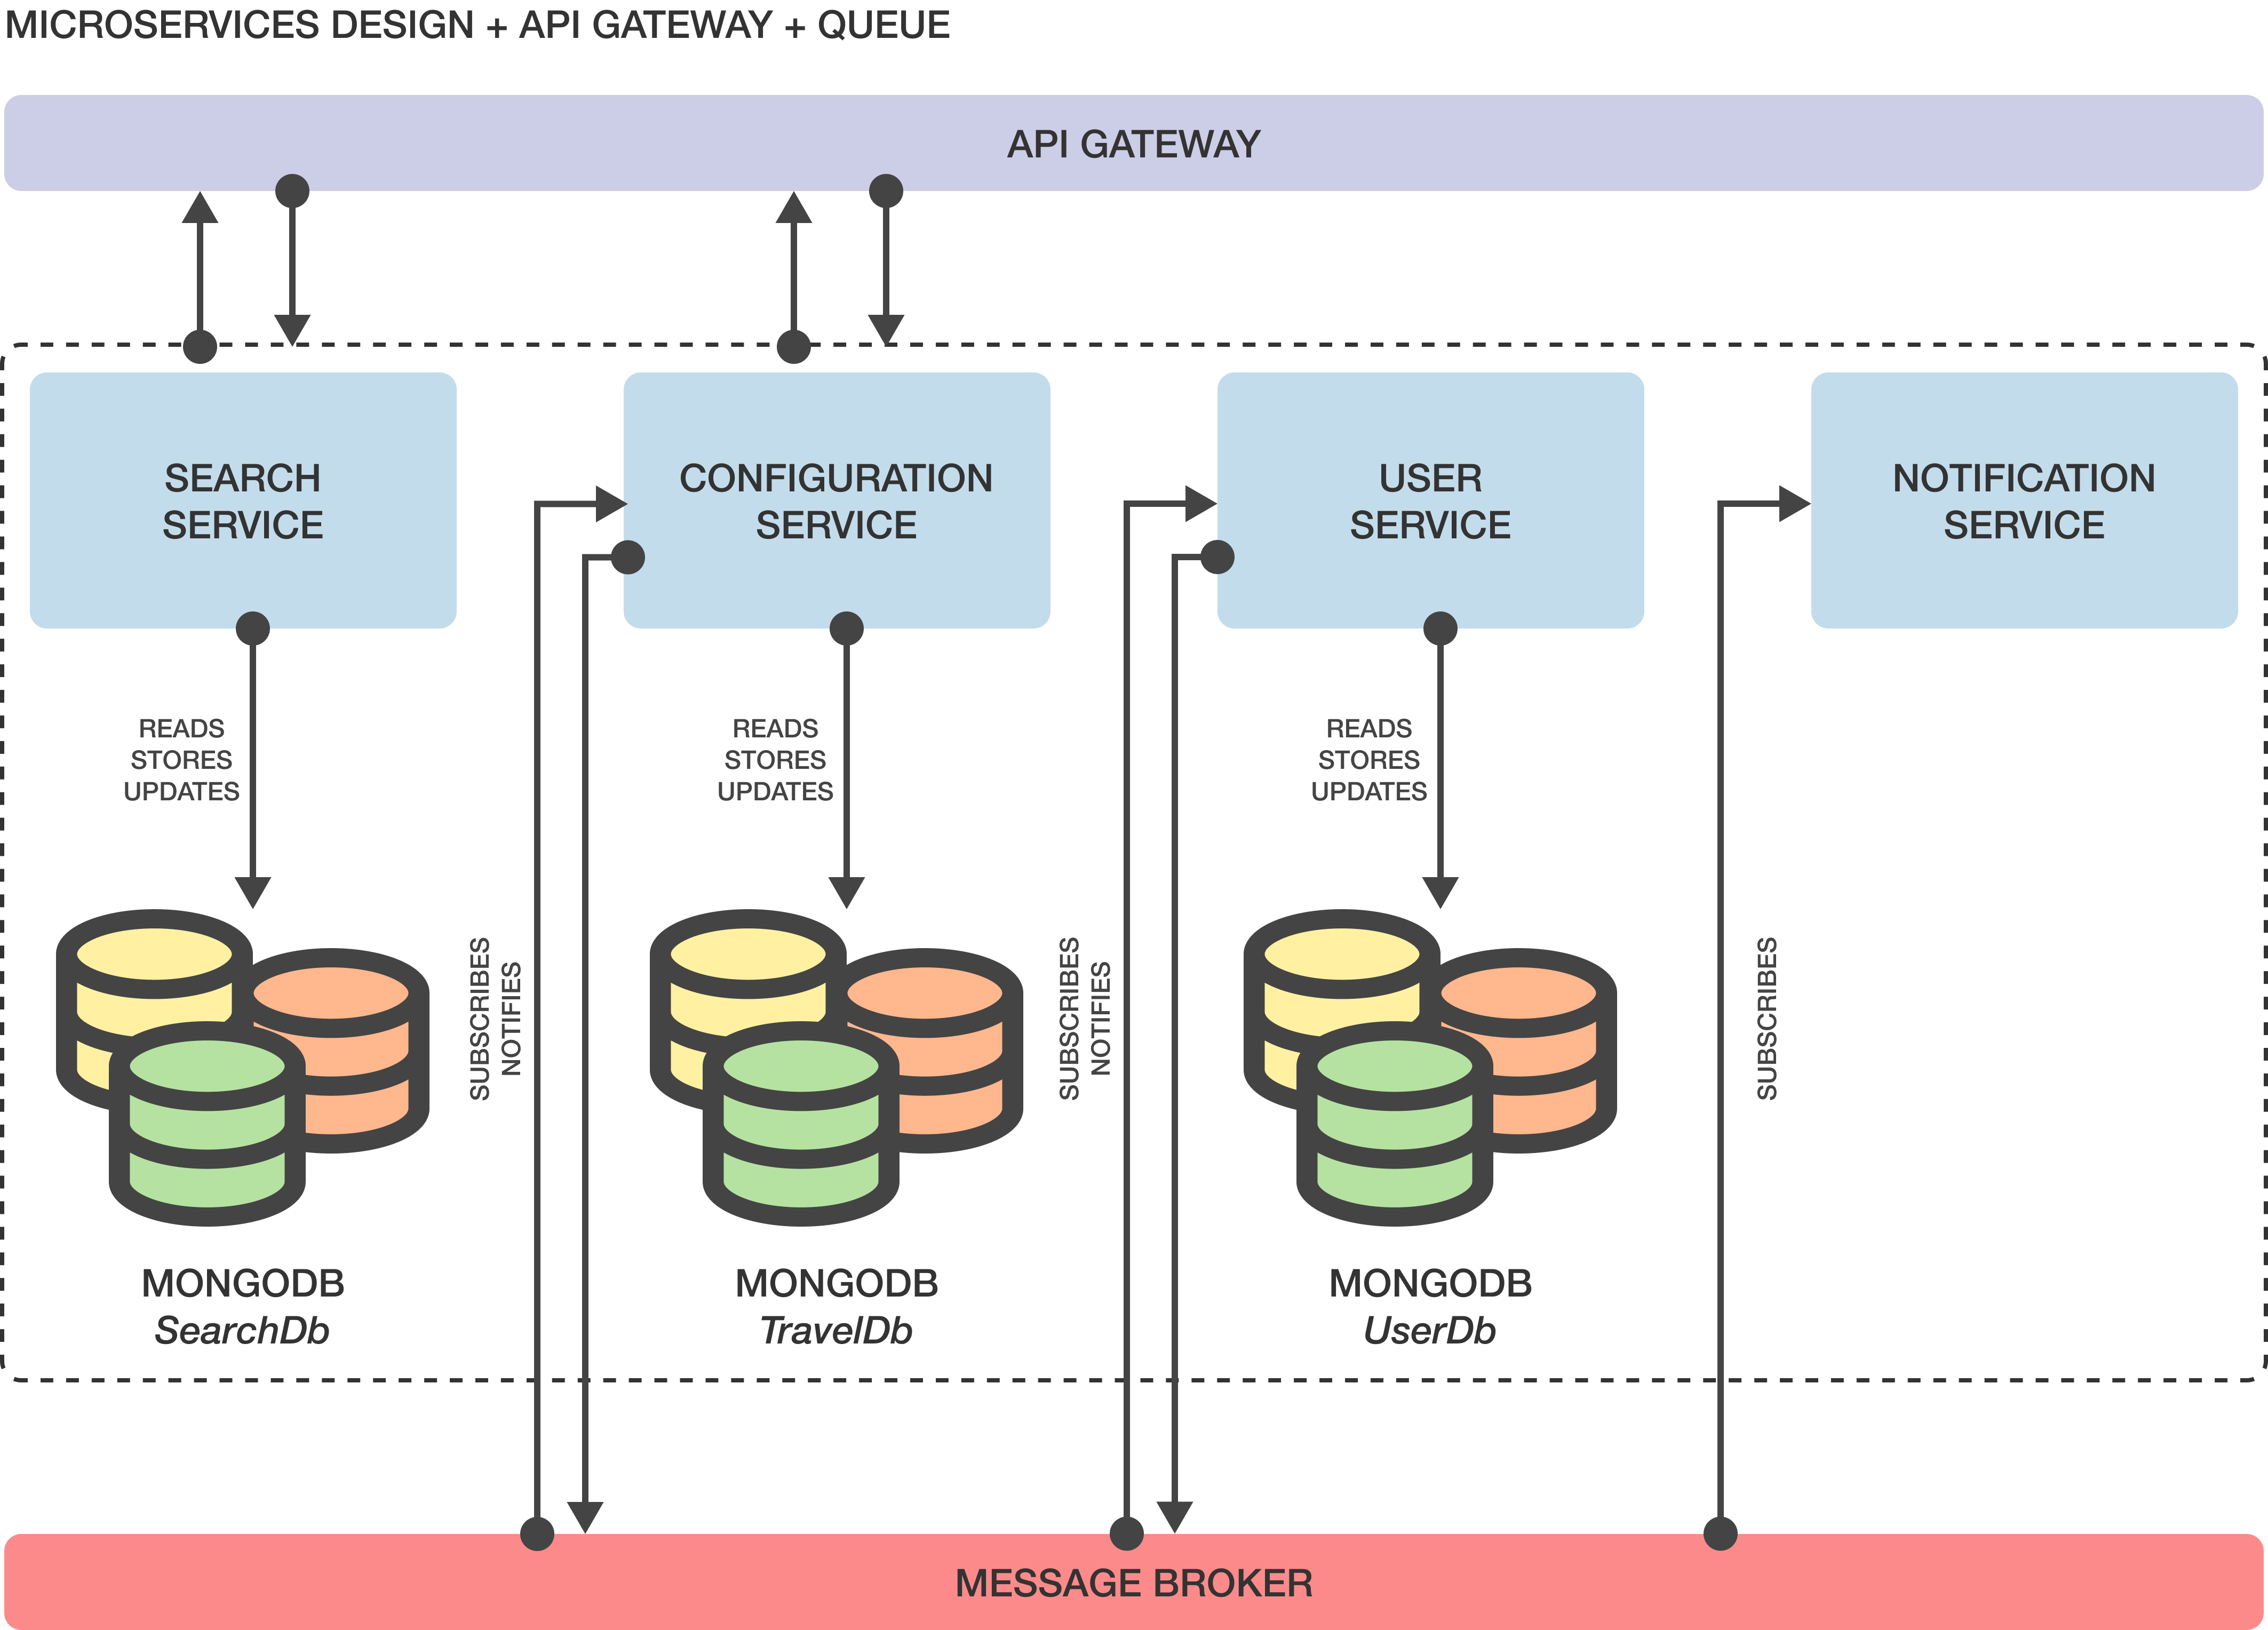
\includegraphics[width=\textwidth]{./assets/microservice-gateway-queue-struct.png}
	\caption{Final architecture design}
\end{figure}
\end{document}
